\documentclass{article}\usepackage[]{graphicx}\usepackage[]{color}
% maxwidth is the original width if it is less than linewidth
% otherwise use linewidth (to make sure the graphics do not exceed the margin)
\makeatletter
\def\maxwidth{ %
  \ifdim\Gin@nat@width>\linewidth
    \linewidth
  \else
    \Gin@nat@width
  \fi
}
\makeatother

\definecolor{fgcolor}{rgb}{0.345, 0.345, 0.345}
\newcommand{\hlnum}[1]{\textcolor[rgb]{0.686,0.059,0.569}{#1}}%
\newcommand{\hlstr}[1]{\textcolor[rgb]{0.192,0.494,0.8}{#1}}%
\newcommand{\hlcom}[1]{\textcolor[rgb]{0.678,0.584,0.686}{\textit{#1}}}%
\newcommand{\hlopt}[1]{\textcolor[rgb]{0,0,0}{#1}}%
\newcommand{\hlstd}[1]{\textcolor[rgb]{0.345,0.345,0.345}{#1}}%
\newcommand{\hlkwa}[1]{\textcolor[rgb]{0.161,0.373,0.58}{\textbf{#1}}}%
\newcommand{\hlkwb}[1]{\textcolor[rgb]{0.69,0.353,0.396}{#1}}%
\newcommand{\hlkwc}[1]{\textcolor[rgb]{0.333,0.667,0.333}{#1}}%
\newcommand{\hlkwd}[1]{\textcolor[rgb]{0.737,0.353,0.396}{\textbf{#1}}}%
\let\hlipl\hlkwb

\usepackage{framed}
\makeatletter
\newenvironment{kframe}{%
 \def\at@end@of@kframe{}%
 \ifinner\ifhmode%
  \def\at@end@of@kframe{\end{minipage}}%
  \begin{minipage}{\columnwidth}%
 \fi\fi%
 \def\FrameCommand##1{\hskip\@totalleftmargin \hskip-\fboxsep
 \colorbox{shadecolor}{##1}\hskip-\fboxsep
     % There is no \\@totalrightmargin, so:
     \hskip-\linewidth \hskip-\@totalleftmargin \hskip\columnwidth}%
 \MakeFramed {\advance\hsize-\width
   \@totalleftmargin\z@ \linewidth\hsize
   \@setminipage}}%
 {\par\unskip\endMakeFramed%
 \at@end@of@kframe}
\makeatother

\definecolor{shadecolor}{rgb}{.97, .97, .97}
\definecolor{messagecolor}{rgb}{0, 0, 0}
\definecolor{warningcolor}{rgb}{1, 0, 1}
\definecolor{errorcolor}{rgb}{1, 0, 0}
\newenvironment{knitrout}{}{} % an empty environment to be redefined in TeX

\usepackage{alltt}
\usepackage[sc]{mathpazo}
\renewcommand{\sfdefault}{lmss}
\renewcommand{\ttdefault}{lmtt}
\usepackage[T1]{fontenc}
\usepackage{geometry}
\geometry{verbose,tmargin=2.5cm,bmargin=2.5cm,lmargin=2.5cm,rmargin=2.5cm}
\setcounter{secnumdepth}{2}
\setcounter{tocdepth}{2}
\usepackage[unicode=true,pdfusetitle,
 bookmarks=true,bookmarksnumbered=true,bookmarksopen=true,bookmarksopenlevel=2,
 breaklinks=false,pdfborder={0 0 1},backref=false,colorlinks=false]
 {hyperref}
\hypersetup{
 pdfstartview={XYZ null null 1}}

\makeatletter
%%%%%%%%%%%%%%%%%%%%%%%%%%%%%% User specified LaTeX commands.
\renewcommand{\textfraction}{0.05}
\renewcommand{\topfraction}{0.8}
\renewcommand{\bottomfraction}{0.8}
\renewcommand{\floatpagefraction}{0.75}

\makeatother
\IfFileExists{upquote.sty}{\usepackage{upquote}}{}
\begin{document}








The results below are generated from an R script.

\begin{knitrout}
\definecolor{shadecolor}{rgb}{0.969, 0.969, 0.969}\color{fgcolor}\begin{kframe}
\begin{alltt}
\hlstd{list.of.packages} \hlkwb{<-} \hlkwd{c}\hlstd{(}\hlstr{"pracma"}\hlstd{)}
\hlstd{new.packages} \hlkwb{<-} \hlstd{list.of.packages[}\hlopt{!}\hlstd{(list.of.packages} \hlopt \hlkwd{installed.packages}\hlstd{()[,}\hlstr{"Package"}\hlstd{])]}
\hlkwa{if}\hlstd{(}\hlkwd{length}\hlstd{(new.packages))} \hlkwd{install.packages}\hlstd{(new.packages)}

\hlkwd{library}\hlstd{(pracma)}
\hlkwd{library}\hlstd{(ggplot2)}

\hlcom{## Formel für Dichtefunktion von V und Verteilungsfunktion von V bzw. P(Gesamtrendite \textbackslash{}in  (l,h)). Herleitung siehe Uebungsblatt 13.}

\hlstd{Density_fun} \hlkwb{<-} \hlkwa{function}\hlstd{(}\hlkwc{v}\hlstd{)\{}

  \hlstd{term_1} \hlkwb{=} \hlopt{-}\hlnum{13} \hlopt{+} \hlnum{2}\hlopt{*}\hlstd{v}
  \hlstd{term_2} \hlkwb{=} \hlopt{-}\hlnum{16} \hlopt{+} \hlnum{2}\hlopt{*}\hlstd{v}

  \hlstd{sum_all} \hlkwb{=} \hlkwd{pnorm}\hlstd{(term_1)} \hlopt{-} \hlkwd{pnorm}\hlstd{(term_2)}
  \hlkwd{return}\hlstd{(}\hlnum{2}\hlopt{/}\hlnum{3} \hlopt{*} \hlstd{sum_all)}

\hlstd{\}}

\hlstd{x} \hlkwb{<-} \hlkwd{seq}\hlstd{(}\hlnum{4.5}\hlstd{,}\hlnum{10.5}\hlstd{,}\hlkwc{by}\hlstd{=}\hlnum{0.05}\hlstd{)}
\hlstd{y} \hlkwb{<-} \hlkwd{Density_fun_2}\hlstd{(x)}
\hlkwd{plot}\hlstd{(x, y,} \hlkwc{type} \hlstd{=}\hlstr{"l"}\hlstd{)}
\end{alltt}
\end{kframe}

{\centering 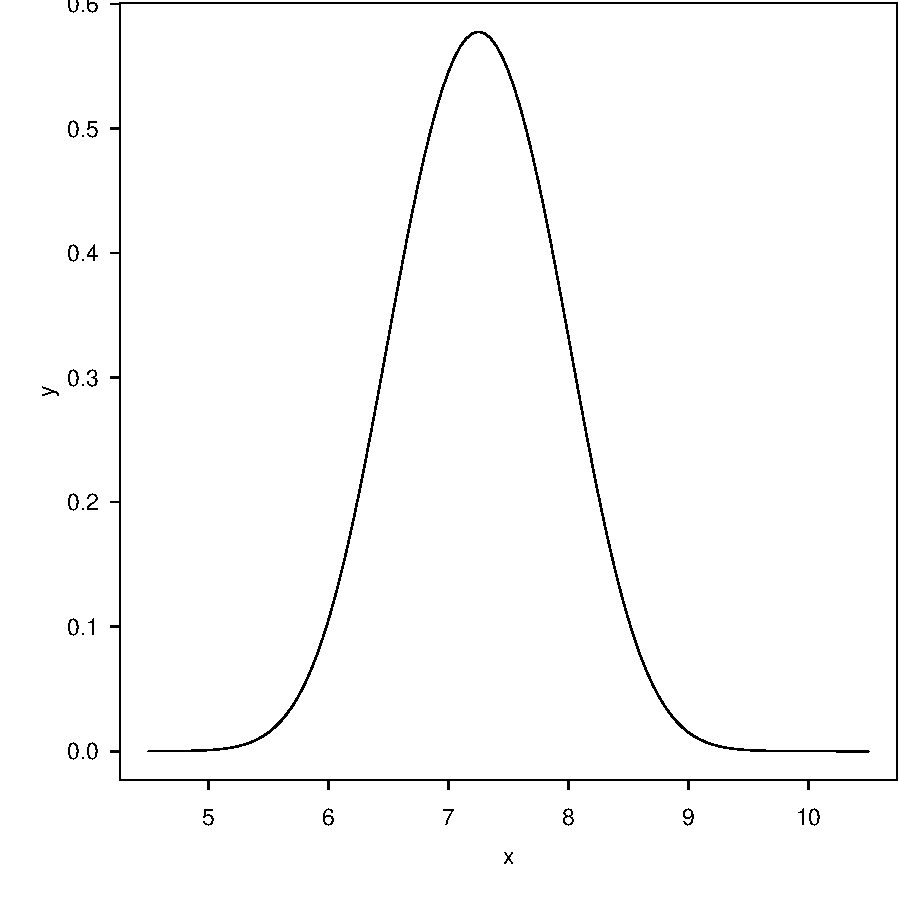
\includegraphics[width=.6\linewidth]{figure/Rendite-Rnwauto-report-1} 

}


\begin{kframe}\begin{alltt}
\hlstd{Prob_dist} \hlkwb{<-} \hlkwa{function}\hlstd{(}\hlkwc{l}\hlstd{=}\hlopt{-}\hlnum{1000}\hlstd{,}\hlkwc{h}\hlstd{)\{}

  \hlstd{ah} \hlkwb{=} \hlopt{-}\hlnum{13}\hlopt{+}\hlnum{2}\hlopt{*}\hlstd{h}
  \hlstd{al} \hlkwb{=} \hlopt{-}\hlnum{13}\hlopt{+}\hlnum{2}\hlopt{*}\hlstd{l}
  \hlstd{bh} \hlkwb{=} \hlopt{-}\hlnum{16}\hlopt{+}\hlnum{2}\hlopt{*}\hlstd{h}
  \hlstd{bl} \hlkwb{=} \hlopt{-}\hlnum{16}\hlopt{+}\hlnum{2}\hlopt{*}\hlstd{l}

  \hlstd{term_ah} \hlkwb{=} \hlstd{ah} \hlopt{*} \hlkwd{pnorm}\hlstd{(ah)} \hlopt{+} \hlkwd{exp}\hlstd{(}\hlopt{-}\hlstd{(ah}\hlopt{^}\hlnum{2}\hlstd{)}\hlopt{/}\hlnum{2}\hlstd{)}\hlopt{/}\hlkwd{sqrt}\hlstd{(}\hlnum{2}\hlopt{*}\hlstd{pi)}
  \hlstd{term_al} \hlkwb{=} \hlstd{al} \hlopt{*} \hlkwd{pnorm}\hlstd{(al)} \hlopt{+} \hlkwd{exp}\hlstd{(}\hlopt{-}\hlstd{(al}\hlopt{^}\hlnum{2}\hlstd{)}\hlopt{/}\hlnum{2}\hlstd{)}\hlopt{/}\hlkwd{sqrt}\hlstd{(}\hlnum{2}\hlopt{*}\hlstd{pi)}
  \hlstd{term_bh} \hlkwb{=} \hlstd{bh} \hlopt{*} \hlkwd{pnorm}\hlstd{(bh)} \hlopt{+} \hlkwd{exp}\hlstd{(}\hlopt{-}\hlstd{(bh}\hlopt{^}\hlnum{2}\hlstd{)}\hlopt{/}\hlnum{2}\hlstd{)}\hlopt{/}\hlkwd{sqrt}\hlstd{(}\hlnum{2}\hlopt{*}\hlstd{pi)}
  \hlstd{term_bl} \hlkwb{=} \hlstd{bl} \hlopt{*} \hlkwd{pnorm}\hlstd{(bl)} \hlopt{+} \hlkwd{exp}\hlstd{(}\hlopt{-}\hlstd{(bl}\hlopt{^}\hlnum{2}\hlstd{)}\hlopt{/}\hlnum{2}\hlstd{)}\hlopt{/}\hlkwd{sqrt}\hlstd{(}\hlnum{2}\hlopt{*}\hlstd{pi)}

  \hlstd{sum_all} \hlkwb{=} \hlstd{term_ah} \hlopt{-} \hlstd{term_al} \hlopt{-} \hlstd{term_bh} \hlopt{+} \hlstd{term_bl}
  \hlkwd{return}\hlstd{(}\hlnum{1}\hlopt{/}\hlnum{3} \hlopt{*} \hlstd{sum_all)}
\hlstd{\}}

\hlcom{# Plots zum veranschaulichen des Unterschieds zwischen Verteilung gemäß Faltung und Normalverteilung}

\hlstd{x}\hlkwb{=}\hlkwd{seq}\hlstd{(}\hlnum{4}\hlstd{,}\hlnum{10}\hlstd{,}\hlkwc{by}\hlstd{=}\hlnum{0.05}\hlstd{)}

\hlstd{df} \hlkwb{<-} \hlkwd{data.frame}\hlstd{(}\hlkwc{v}\hlstd{=x,} \hlkwc{y} \hlstd{=} \hlkwd{Prob_dist}\hlstd{(}\hlkwc{h}\hlstd{=x),} \hlkwc{z} \hlstd{=}  \hlkwd{pnorm}\hlstd{(x,}\hlkwc{mean}\hlstd{=} \hlnum{7.25}\hlstd{,}\hlkwc{sd} \hlstd{=} \hlkwd{sqrt}\hlstd{(}\hlnum{7}\hlopt{/}\hlnum{16}\hlstd{)) )}

\hlkwd{ggplot}\hlstd{(df,} \hlkwd{aes}\hlstd{(}\hlkwc{x}\hlstd{=v))}\hlopt{+}
  \hlkwd{geom_line}\hlstd{(}\hlkwd{aes}\hlstd{(}\hlkwc{y}\hlstd{=y),}\hlkwc{color} \hlstd{=} \hlstr{"blue"}\hlstd{)}\hlopt{+} \hlcom{#Verteilungsfunktion von V}
  \hlkwd{geom_line}\hlstd{(}\hlkwd{aes}\hlstd{(}\hlkwc{y}\hlstd{=z),}\hlkwc{color} \hlstd{=} \hlstr{"red"}\hlstd{)}   \hlcom{#Verteilungsfunktion der Normalverteilung mit \textbackslash{}mu = E(V) und \textbackslash{}sigma^2 = Var(V)}
\end{alltt}
\end{kframe}

{\centering 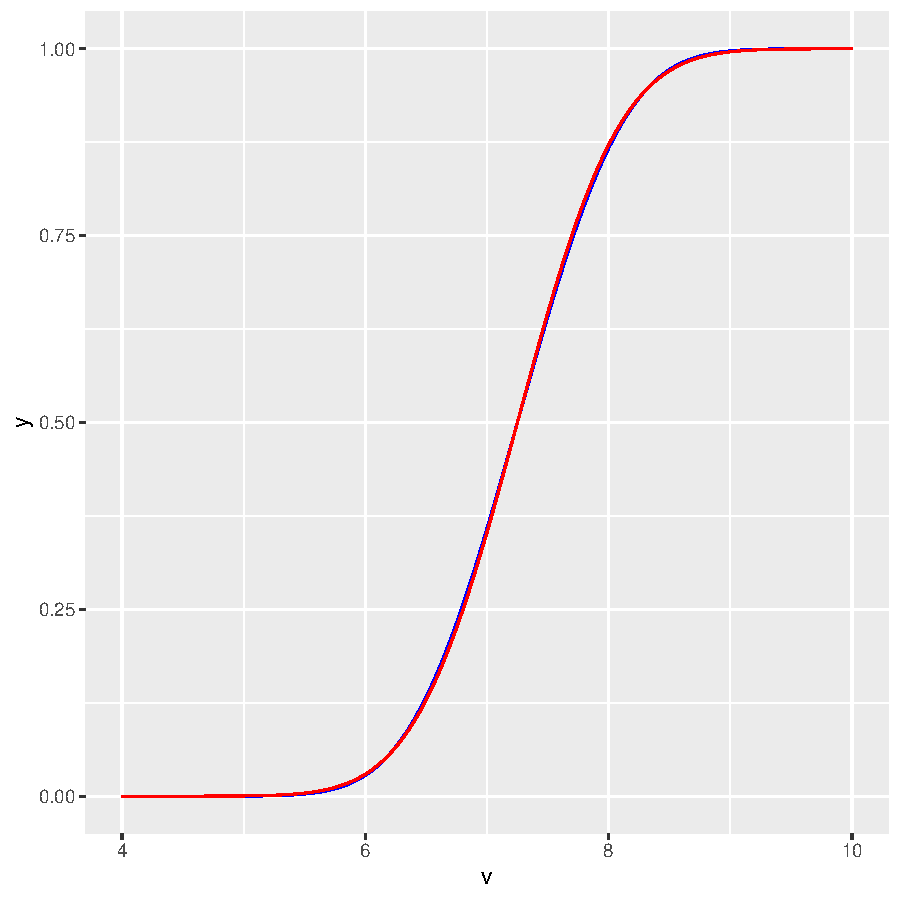
\includegraphics[width=.6\linewidth]{figure/Rendite-Rnwauto-report-2} 

}


\begin{kframe}\begin{alltt}
\hlstd{df2} \hlkwb{<-} \hlkwd{data.frame}\hlstd{(}\hlkwc{v}\hlstd{=x,} \hlkwc{y} \hlstd{=} \hlkwd{Density_fun}\hlstd{(}\hlkwc{v}\hlstd{=x),} \hlkwc{z} \hlstd{=} \hlkwd{dnorm}\hlstd{(x,}\hlkwc{mean}\hlstd{=} \hlnum{7.25}\hlstd{,}\hlkwc{sd} \hlstd{=} \hlkwd{sqrt}\hlstd{(}\hlnum{7}\hlopt{/}\hlnum{16}\hlstd{)) )}

\hlkwd{ggplot}\hlstd{(df2,} \hlkwd{aes}\hlstd{(}\hlkwc{x}\hlstd{=v))}\hlopt{+}
  \hlkwd{geom_line}\hlstd{(}\hlkwd{aes}\hlstd{(}\hlkwc{y}\hlstd{=y),}\hlkwc{color} \hlstd{=} \hlstr{"blue"}\hlstd{)}\hlopt{+}  \hlcom{#Dichtefunktion von V}
  \hlkwd{geom_line}\hlstd{(}\hlkwd{aes}\hlstd{(}\hlkwc{y}\hlstd{=z),}\hlkwc{color} \hlstd{=} \hlstr{"red"}\hlstd{)}    \hlcom{#Dichtefunktion der Normalverteilung mit \textbackslash{}mu = E(V) und \textbackslash{}sigma^2 = Var(V)}
\end{alltt}
\end{kframe}

{\centering 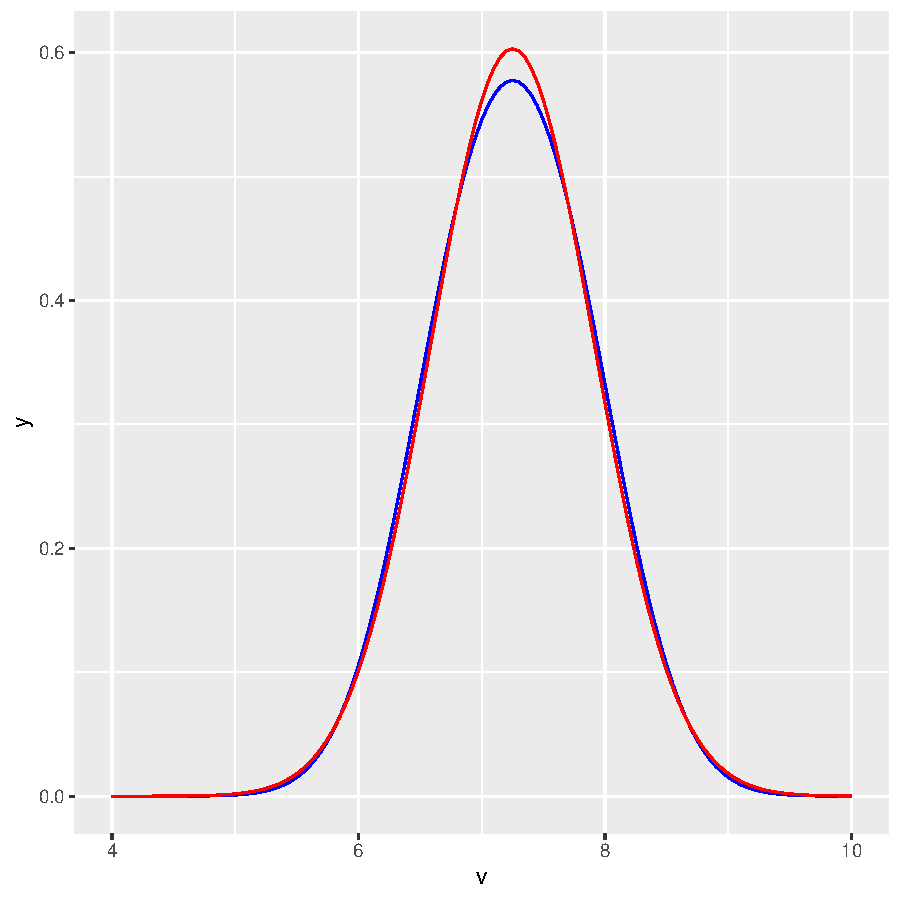
\includegraphics[width=.6\linewidth]{figure/Rendite-Rnwauto-report-3} 

}


\begin{kframe}\begin{alltt}
\hlcom{## Gleiche Verteilungen/Dichten, bloss mit erf-function berechnet.}

\hlstd{Density_fun_erf} \hlkwb{<-} \hlkwa{function}\hlstd{(}\hlkwc{v}\hlstd{)\{}

  \hlstd{term_1} \hlkwb{=} \hlkwd{sqrt}\hlstd{(}\hlnum{2}\hlstd{)}\hlopt{*}\hlstd{(}\hlopt{-}\hlnum{6.5} \hlopt{+} \hlstd{v)}
  \hlstd{term_2} \hlkwb{=} \hlkwd{sqrt}\hlstd{(}\hlnum{2}\hlstd{)}\hlopt{*}\hlstd{(}\hlopt{-}\hlnum{8} \hlopt{+} \hlstd{v)}

  \hlstd{sum_all} \hlkwb{=} \hlkwd{erf}\hlstd{(term_1)}\hlopt{-} \hlkwd{erf}\hlstd{(term_2)}
  \hlkwd{return}\hlstd{(}\hlnum{1}\hlopt{/}\hlnum{3} \hlopt{*} \hlstd{sum_all)}

\hlstd{\}}



\hlstd{Prob_dist_erf} \hlkwb{<-} \hlkwa{function}\hlstd{(}\hlkwc{l}\hlstd{=}\hlopt{-}\hlnum{1000}\hlstd{,}\hlkwc{h}\hlstd{)\{}

  \hlstd{ah} \hlkwb{=} \hlkwd{sqrt}\hlstd{(}\hlnum{2}\hlstd{)}\hlopt{*}\hlstd{(}\hlopt{-}\hlnum{6.5} \hlopt{+} \hlstd{h)}
  \hlstd{al} \hlkwb{=} \hlkwd{sqrt}\hlstd{(}\hlnum{2}\hlstd{)}\hlopt{*}\hlstd{(}\hlopt{-}\hlnum{6.5} \hlopt{+} \hlstd{l)}
  \hlstd{bh} \hlkwb{=} \hlkwd{sqrt}\hlstd{(}\hlnum{2}\hlstd{)}\hlopt{*}\hlstd{(}\hlopt{-}\hlnum{8} \hlopt{+} \hlstd{h)}
  \hlstd{bl} \hlkwb{=} \hlkwd{sqrt}\hlstd{(}\hlnum{2}\hlstd{)}\hlopt{*}\hlstd{(}\hlopt{-}\hlnum{8} \hlopt{+} \hlstd{l)}

  \hlstd{term_ah} \hlkwb{=} \hlstd{ah} \hlopt{*} \hlkwd{erf}\hlstd{(ah)} \hlopt{+} \hlkwd{exp}\hlstd{(}\hlopt{-}\hlstd{ah}\hlopt{^}\hlnum{2}\hlstd{)}\hlopt{/}\hlkwd{sqrt}\hlstd{(pi)}
  \hlstd{term_al} \hlkwb{=} \hlstd{al} \hlopt{*} \hlkwd{erf}\hlstd{(al)} \hlopt{+} \hlkwd{exp}\hlstd{(}\hlopt{-}\hlstd{al}\hlopt{^}\hlnum{2}\hlstd{)}\hlopt{/}\hlkwd{sqrt}\hlstd{(pi)}
  \hlstd{term_bh} \hlkwb{=} \hlstd{bh} \hlopt{*} \hlkwd{erf}\hlstd{(bh)} \hlopt{+} \hlkwd{exp}\hlstd{(}\hlopt{-}\hlstd{bh}\hlopt{^}\hlnum{2}\hlstd{)}\hlopt{/}\hlkwd{sqrt}\hlstd{(pi)}
  \hlstd{term_bl} \hlkwb{=} \hlstd{bl} \hlopt{*} \hlkwd{erf}\hlstd{(bl)} \hlopt{+} \hlkwd{exp}\hlstd{(}\hlopt{-}\hlstd{bl}\hlopt{^}\hlnum{2}\hlstd{)}\hlopt{/}\hlkwd{sqrt}\hlstd{(pi)}

  \hlstd{sum_all} \hlkwb{=} \hlstd{term_ah} \hlopt{-} \hlstd{term_al} \hlopt{-} \hlstd{term_bh} \hlopt{+} \hlstd{term_bl}
  \hlkwd{return}\hlstd{(}\hlnum{1}\hlopt{/}\hlnum{3} \hlopt{*} \hlnum{1}\hlopt{/}\hlkwd{sqrt}\hlstd{(}\hlnum{2}\hlstd{)} \hlopt{*} \hlstd{sum_all)}
\hlstd{\}}
\end{alltt}
\end{kframe}
\end{knitrout}

The R session information (including the OS info, R version and all
packages used):

\begin{knitrout}
\definecolor{shadecolor}{rgb}{0.969, 0.969, 0.969}\color{fgcolor}\begin{kframe}
\begin{alltt}
\hlkwd{sessionInfo}\hlstd{()}
\end{alltt}
\begin{verbatim}
## R version 4.0.4 (2021-02-15)
## Platform: x86_64-apple-darwin17.0 (64-bit)
## Running under: macOS 12.1
## 
## Matrix products: default
## LAPACK: /Library/Frameworks/R.framework/Versions/4.0/Resources/lib/libRlapack.dylib
## 
## locale:
## [1] de_CH.UTF-8/de_CH.UTF-8/de_CH.UTF-8/C/de_CH.UTF-8/de_CH.UTF-8
## 
## attached base packages:
## [1] stats     graphics  grDevices utils     datasets  methods   base     
## 
## other attached packages:
## [1] ggplot2_3.3.5 pracma_2.3.6 
## 
## loaded via a namespace (and not attached):
##  [1] knitr_1.36       magrittr_2.0.1   tidyselect_1.1.1 munsell_0.5.0    colorspace_2.0-2
##  [6] R6_2.5.1         rlang_0.4.12     fansi_0.5.0      highr_0.9        stringr_1.4.0   
## [11] dplyr_1.0.7      tools_4.0.4      grid_4.0.4       gtable_0.3.0     xfun_0.29       
## [16] utf8_1.2.2       DBI_1.1.1        withr_2.4.3      ellipsis_0.3.2   digest_0.6.29   
## [21] assertthat_0.2.1 tibble_3.1.6     lifecycle_1.0.1  crayon_1.4.2     farver_2.1.0    
## [26] purrr_0.3.4      vctrs_0.3.8      evaluate_0.14    glue_1.6.0       labeling_0.4.2  
## [31] stringi_1.7.6    compiler_4.0.4   pillar_1.6.4     generics_0.1.1   scales_1.1.1    
## [36] pkgconfig_2.0.3
\end{verbatim}
\begin{alltt}
\hlkwd{Sys.time}\hlstd{()}
\end{alltt}
\begin{verbatim}
## [1] "2022-01-29 18:13:50 CET"
\end{verbatim}
\end{kframe}
\end{knitrout}


\end{document}
